\documentclass[11pt,aspectratio=169]{beamer}

% -------------------- THEME & LAYOUT --------------------
\usetheme{Madrid}
\usecolortheme{dolphin} % base color scheme
\usefonttheme{professionalfonts}
\setbeamercovered{transparent}
\setbeamertemplate{navigation symbols}{}   % remove navigation buttons
\setbeamertemplate{caption}[numbered]      % numbered captions
\setbeamertemplate{itemize items}[triangle]
\setbeamersize{text margin left=1.2cm,text margin right=1.2cm} % adjust to taste

% -------------------- GLOBAL FONT SETTINGS --------------------

% 1. Force the base beamer font to small
\setbeamerfont{normal text}{size=\small}

% 2. Force math environments to follow the "small" font size
\setbeamerfont{math text}{size=\small}
\setbeamerfont{equation}{size=\small}

% 3. Redefine \normalsize itself 
% This ensures equations and lists (which look for \normalsize) use  instead.
\let\oldnormalsize\normalsize
\renewcommand{\normalsize}{\oldnormalsize\small}

% 4. Ensure lists also stay small
\setbeamerfont{itemize/enumerate body}{size=\small}
\setbeamerfont{itemize/enumerate subbody}{size=\small}


% -------------------- FONTS & TYPOGRAPHY --------------------
\usepackage[T1]{fontenc}
\usepackage[utf8]{inputenc}
\usepackage{newpxtext,newpxmath} % Palatino-like font & math
\usepackage{microtype}

% -------------------- MATH, TABLES & GRAPHICS --------------------
\usepackage{amsmath,amssymb,amsfonts,mathtools}
\usepackage{bm,booktabs,siunitx,graphicx}
\graphicspath{{./}{./figures/}}
\renewcommand{\theequation}{3.\arabic{equation}}

% -------------------- UTILITIES --------------------
\usepackage{appendixnumberbeamer}
\usepackage{ragged2e}
\usepackage{xspace}
\usepackage{csquotes}
% -------------------- Bibliography --------------------
\usepackage[style=authoryear-comp]{biblatex} % 'comp' stands for condensed/compressed
\addbibresource{sources.bib}
\usepackage{xcolor}

% -------------------- HYPERREF --------------------
\hypersetup{
  colorlinks=false,
  pdfauthor={Francesca},
  pdftitle={Chapter 1 — The Value of Currency}
}

% -------------------- COLORS & EMPHASIS --------------------
\definecolor{myblue}{RGB}{0,70,140}
\definecolor{myred}{RGB}{180,30,30}
\definecolor{mygreen}{RGB}{0,120,70}
\definecolor{gold}{RGB}{184,134,11}

\setbeamercolor{title}{fg=gold}       % title page
\setbeamercolor{frametitle}{fg=gold}  % slide titles
\setbeamercolor{structure}{fg=gold}   % bullets, sections, links
\setbeamercolor{section in head/foot}{fg=gold,bg=black!10} % gold text on light background

% -------------------- FOOTLINE --------------------
\setbeamertemplate{footline}{
  \leavevmode%
  \hbox{%
    % Section links (hidden if no current section)
    \begin{beamercolorbox}[wd=0.7\paperwidth,ht=2.5ex,dp=1.5ex,leftskip=1.4em]{section in head/foot}%
      \ifx\insertsection\empty
        % nothing
      \else
        Section: \insertsection
      \fi
    \end{beamercolorbox}%
    % Frame number right
    \begin{beamercolorbox}[wd=0.3\paperwidth,ht=2.5ex,dp=1.5ex,leftskip=3.8cm]{section in head/foot}%
      \insertframenumber/\inserttotalframenumber
    \end{beamercolorbox}%
  }%
  \vskip1pt%
}



\newcommand{\highlight}[1]{\textcolor{myblue}{#1}}
\newcommand{\warning}[1]{\textcolor{myred}{#1}}

% -------------------- SHORTCUTS --------------------
\newcommand{\E}{\mathbb{E}}
\newcommand{\R}{\mathbb{R}}
\newcommand{\dd}{\mathrm{d}}
\newcommand{\mc}[1]{\mathcal{#1}}
\newcommand{\bb}[1]{\mathbb{#1}}
\newcommand{\uc}{U_c}
\newcommand{\zg}{Z_g}

% -------------------- TIGHTER DISPLAY MATH --------------------
\makeatletter
\g@addto@macro\normalsize{%
  \setlength\abovedisplayskip{8pt}%
  \setlength\belowdisplayskip{8pt}%
  \setlength\abovedisplayshortskip{6pt}%
  \setlength\belowdisplayshortskip{6pt}%
}
\makeatother
\setbeamertemplate{frametitle}{
  \nointerlineskip
  \begin{beamercolorbox}[wd=\paperwidth,ht=3.5ex,dp=1ex,center]{frametitle}
    \centering\insertframetitle
  \end{beamercolorbox}
}

% -------------------- METADATA --------------------
\title[Part I — Currency and Money]{\textbf{Part I: Currency and Money}\\[2pt]\large Chapter 1 — The Value of Currency}
\subtitle{Currency, Money, and Price-Level Determination}
\author{Francesca}
\institute{}
\date{\today}

% -------------------- SECTION ROADMAP --------------------
\AtBeginSection[]
{
  \begin{frame}
    \tableofcontents[currentsection, hideothersubsections]
  \end{frame}
}


\begin{document}
\setcounter{equation}{0}


% ===================== TITLE SLIDE =====================
\begin{frame}[plain] % 'plain' removes header/footer for the title slide

\begin{columns}[T,totalwidth=\textwidth]

% ----- Left column: Main title, professor, chapter -----
\begin{column}{0.45\textwidth}
\vspace{2cm}

% Main title
{\usebeamercolor[fg]{title}\LARGE\textbf{Monetary Economics}\\[0.3cm]
\LARGE\textbf{and Policy}} 

\vspace{0.5cm}

% Professor name and date
{\large\textit{Pierpaolo Benigno}}\\[0.1cm]

\vspace{1cm}

% Chapter and subtitle
{\usebeamercolor[fg]{frametitle}\large Chapter 3: Central Bank Digital Currency}

\end{column}

% ----- Right column: Image -----
\begin{column}{0.55\textwidth}
\vspace{1cm}
\centering
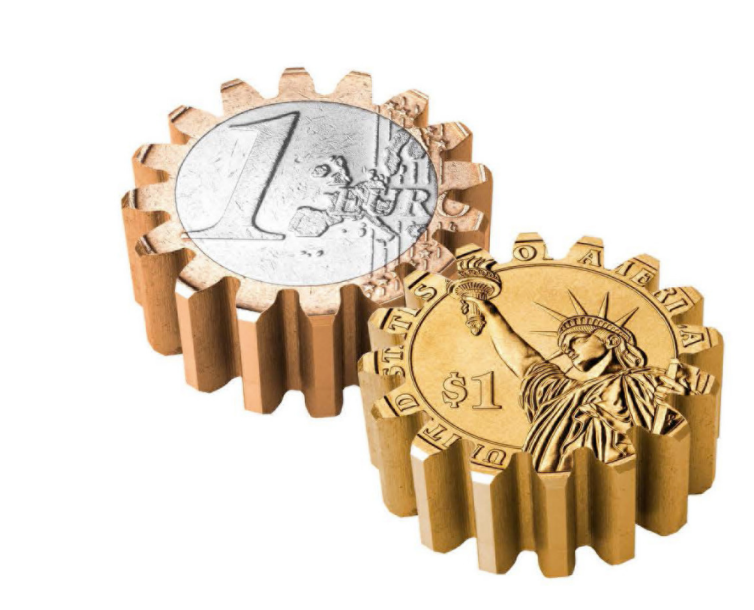
\includegraphics[width=0.9\linewidth]{Cover.png}
\end{column}

\end{columns}

% ----- Footer text (bottom-right corner) -----
\vspace*{2cm} % adjust if needed
\hfill{\large\textit{Prepared by Marcos Consuegra}}

\end{frame}

\begin{frame}{What We Will Learn}
\small

\begin{itemize}
  \item How \textbf{CBDCs} make central bank liabilities \textbf{provide liquidity services}.
  \item Why this creates a \textbf{spread} between the \textbf{policy rate} and the \textbf{market rate.}
\end{itemize}

\vspace{0.5em}

\begin{itemize}
  \item How both the \textbf{policy rate} and the \textbf{stock of reserves} \textbf{affect inflation.}
  \item When the model nests the price-level mechanism of Chapter~1.
\end{itemize}

\vspace{0.5em}

\begin{itemize}
  \item Why \textbf{optimal policy} implies supplying enough liquidity to \textbf{eliminate the spread}.
  \item How the central bank can still \textbf{set inflation} through its \textbf{policy rate}.
\end{itemize}

\vspace{0.5em}

\begin{itemize}
  \item Treasury-backed liquidity and \textbf{the role of fiscal capacity} in price determination.
\end{itemize}

\end{frame}

% OUTLINE
\begin{frame}{Outline}
\tableofcontents
\end{frame}
\section{Introduction}

\begin{frame}{From Crypto to CBDCs: Why This Matters}
\small

\textbf{Context}
\begin{itemize}
  \item Since Bitcoin’s launch in 2009, digital currencies have proliferated, attracting the attention of investors, media, and policymakers.
  \item Their novelty does not lie in making payments digital (already possible via cards and bank accounts), but in enabling \emph{decentralized verification} via blockchain, allowing a degree of cash-like anonymity without requiring third-party validation.
\end{itemize}

\vspace{0.8em}

\textbf{Payment System}
\begin{itemize}
  \item Modern payments are almost fully digital, a significant departure from historical systems where money circulated only in physical form.
  \item As \textcite{cipolla1956} observed, in the early Middle Ages “any commodity could serve as a means of exchange, and coins were just one among many”.
  \item The dominance of a single, government-issued currency—\textbf{monetary sovereignty}—is therefore a relatively recent development.
\end{itemize}

\end{frame}


% --- SLIDE 2 ---
\begin{frame}{The Return of Currency Competition}
\small

\textbf{Historical Note}
\begin{itemize}
  \item Multiple currencies and payment instruments have historically coexisted within the same economy.\footnote{\tiny See also \textcite{cipolla1956, cipolla1982, cipolla1990}.}
  \item Today, digital assets and global payment platforms are reviving \emph{currency competition}.
\end{itemize}

\vspace{0.8em}
\textbf{Implications for Central Banks (CBs)}
\begin{itemize}
  \item Competing currencies can erode seigniorage and weaken CBs' control over money’s value, especially if settlement ceases to occur in the domestic unit.  
  \item In response, CBs are exploring \textbf{Central Bank Digital Currencies (CBDCs)}.
\end{itemize}
\end{frame}

% --- SLIDE 3 ---
\begin{frame}{CBDC Form 1: Digital Tokens}
\small

\textbf{(1) CBDC as Digital Tokens replacing Physical Cash}
\begin{itemize}
  \item Digital tokens represent CB liabilities that store units of account like cash, but their face value could be \textbf{digitally adjusted} by the issuer over time.  
  \item When tokens serve as the store of value, \emph{no-arbitrage} prevents $i_t^X < 0$.
  \item However, such tokens can \textbf{relax the zero lower bound (ZLB)} by allowing negative interest rates.
  \item Still, \textbf{price-level control} with tokens alone remains as in Chapters~1–2; novel effects arise when reserves both \textbf{pay interest} and \textbf{provide liquidity}.
\end{itemize}
\end{frame}


% --- SLIDE 4 ---
\begin{frame}{CBDC Form 2: Retail Access to Central Bank Reserves}
\small

\textbf{(2) CBDC as Interest-Bearing, Liquidity-Providing Money}
\begin{itemize}
  \item In this form, the CBDC is modeled as \textbf{interest-bearing deposits} at the CB that are directly accessible to households.
  \item These deposits serve as \emph{money-like securities}: they provide \textbf{liquidity services} that can enter household utility and also \textbf{yield interest}.
  \item Introducing these liquidity benefits for interest-bearing reserves alters the mechanism of \textbf{price-level determination} discussed in Chapter~2.
  \item Whether or not digital tokens circulate is largely irrelevant for this mechanism (under perfect substitutability); \textbf{tokens mainly affect the ZLB}.
\end{itemize}
\end{frame}

\begin{frame}{Outline of the Chapter’s Results}
\small

\textbf{Price-Level Control}  
\begin{itemize}
  \item Inflation depends on both the \textbf{policy rate} and the \textbf{quantity of reserves}, extending the transmission mechanisms discussed in Chapter~1.
\end{itemize}

\textbf{Optimal Liquidity Supply}  
\begin{itemize}
  \item The CB can achieve the \textbf{optimal supply of liquidity} without affecting the interest-rate policy, price level, or inflation, provided it holds sufficient assets.
\end{itemize}

\textbf{Fiscal Coordination} 
\begin{itemize} 
  \item Alternatively, optimal liquidity can be achieved through \textbf{coordination with the Treasury}, by backing Treasury liabilities, subject to fiscal capacity.
\end{itemize}

\end{frame}


\section{Model}

\begin{frame}{Model Overview}
\small

\textbf{Economic Setting}
\begin{itemize}
  \item Infinite-horizon, closed economy under perfect foresight
  \item Single consumption good $C$ with constant endowment $Y$
\end{itemize}

\textbf{Agents}
\begin{itemize}
  \item Representative consumer choosing $C_t$, bonds, and liquidity balances
  \item Treasury issuing debt and levying lump-sum taxes
  \item Central Bank (CB) setting the policy rate and managing its balance sheet
\end{itemize}

\textbf{CB Liabilities}
\begin{itemize}
  \item \textbf{Digital Tokens} $M_t$: non–interest-bearing, functioning as digital cash
  \item \textbf{Reserves} $X_t$: interest-bearing deposits at the CB
  \item Both provide liquidity services through $V\!\left(\tfrac{X_t + M_t}{P_t}\right)$
\end{itemize}

\end{frame}

\begin{frame}{Representative Consumer: Preferences}
\small

\textbf{Intertemporal Utility}
\begin{equation}
\sum_{t=t_0}^{\infty}
\beta^{t-t_0}
\left[
U(C_t)
+ V\!\left(\frac{X_t + M_t}{P_t}\right)
\right]
\label{eq:utility_cbdc}
\end{equation}

\textbf{Interpretation}
\begin{itemize}
  \item $\beta \in (0,1)$: discount factor  
  \item $U(C_t)$: concave utility in consumption  
  \item $V(\cdot)$: concave utility in real liquidity services  
  \item Real liquidity: $q_t = \dfrac{X_t + M_t}{P_t}$  
  \item Satiation: $V_q(q_t)=0$ for $q_t \ge \bar q$
\end{itemize}

\textbf{Economic Meaning:}  
Reserves and tokens ease transaction frictions by providing liquidity services. Once $q_t$ reaches $\bar q$, the household is fully satiated and additional liquidity yields no marginal benefit.

\end{frame}

\begin{frame}{Representative Consumer: Budget Constraint}
\small
\textbf{Budget Constraint at time $t$}
\begin{equation}
B_t + X_t + M_t + P_t C_t + T_t
= (1+i_{t-1})B_{t-1} + (1+i_{t-1}^{X})X_{t-1} + M_{t-1} + P_t Y
\label{eq:budget_cbdc}
\end{equation}

\textbf{Interpretation:}
\begin{itemize}
  \item $B_t$: private/treasury bonds, default-free, unit face value, pay interest $i_{t}$
  \item $X_t$: CB reserves, pay interest $i_{t}^{X}$
  \item $M_t$: digital tokens (non-interest-bearing)
  \item $T_t$: lump-sum taxes (if negative, transfers)
\end{itemize}

\textbf{Key Features}
\begin{itemize}
 \item CB's liabilities provide liquidity services.
  \item Private or treasury bonds do \textbf{not} provide liquidity services $\Longrightarrow$ their yield $i$ can differ from the policy rate $i^X$ on reserves.
 \end{itemize}
\end{frame}
\begin{frame}{Liquidity Properties and Model Assumptions}
\small

\textbf{Liquidity Properties}
\begin{itemize}
  \item Both reserves $X_t$ and tokens $M_t$ provide liquidity services through $V(\cdot)$.
  \item When the policy rate on reserves is positive ($i_t^X>0$), reserves strictly dominate tokens as a store of value.
  \item Digital tokens could, in principle, be engineered to carry negative returns 
        (e.g.\ via digital redenomination), thereby relaxing the traditional zero lower bound.
\end{itemize}

\textbf{Modeling Assumption}
\begin{itemize}
  \item For analytical simplicity, we set $M_t=0$ going forward and treat reserves $X_t$ as the sole 
        liquidity-providing asset. We may also allow the policy rate $i_t^X$ to take negative values if needed.
\end{itemize}

\end{frame}

\begin{frame}{Borrowing Constraint}
\small
\textbf{Real Borrowing Limit}
\begin{equation}
-\frac{(1+i_{t-1})B_{t-1}}{P_t} 
\;\le\;
\frac{(1+i_{t-1}^{X})X_{t-1}}{P_t}
+ \sum_{j=0}^{\infty} R_{t,t+j} 
\left( Y - \frac{T_{t+j}}{P_{t+j}} \right)
< \infty,
\label{eq:borrowing_cbdc}
\end{equation}
\hspace{0.65cm} where $R_{t,t+j}$ is the real discount factor from $t+j$ w.r.t. time $t$.

\vspace{0.25cm}
\noindent\textbf{Real discount factor:}
\begin{equation}
R_{t,t+j} = \prod_{i=1}^{j} \frac{1}{1 + r_{t+i-1}}, 
\quad R_{t,t} \equiv 1, 
\quad j \ge 1.
\label{eq:real_discount_fac}
\end{equation}

\begin{itemize} 
    \item Note, that the real interest rate $r$ is defined as $1+r_t \equiv (1+i_t)\frac{P_t}{P_{t+1}}$. 

\end{itemize}
\end{frame}


\begin{frame}[label=borrowing]{Intertemporal Budget Constraint}
\small

\begin{itemize}
    \item An equivalent formulation replaces the borrowing limit \eqref{eq:borrowing_cbdc} with:
\end{itemize}

\vspace{0.25cm}

\textbf{Intertemporal Budget Constraint:}

\begin{equation}
\sum_{t=t_0}^{\infty} 
R_{t_0,t}
\left(
C_t 
+
\underbrace{
\frac{i_t - i_t^{X}}{1+i_t}\frac{X_t}{P_t}
}_{\text{liquidity cost}}
\right)
\le
\frac{(1+i_{t_0-1})B_{t_0-1} 
+ (1+i_{t_0-1}^{X})X_{t_0-1}}{P_{t_0}}
+
\sum_{t=t_0}^{\infty} 
R_{t_0,t}
\left(
Y - \frac{T_t}{P_t}
\right).
\label{eq:ibc_cbdc}
\end{equation}

\begin{itemize}
  \item This extends the Chapter 1 IBC by incorporating the \emph{liquidity cost} 
  of reserves, which captures the opportunity cost of holding liquidity instead 
  of higher-yield bonds.
\end{itemize}

\vspace{0.3cm}

\begin{center}
\hyperlink{borrowing_proof}{\beamerbutton{See Proof in Appendix}}
\end{center}

\end{frame}

\begin{frame}{Representative Consumer: Problem}
\small
\begin{itemize}
    \item The representative consumer chooses sequences 
$\{C_t, B_t, X_t\}_{t=t_0}^\infty$ 
to maximize intertemporal utility at each time $t\geq t_0$:
\end{itemize}
\[
\max_{\{C_t, B_t, X_t\}} \sum_{t=t_0}^{\infty} 
\beta^{t-t_0} 
\left\{
U(C_t) 
+ V\!\left(\frac{X_t}{P_t}\right)
\right\}.
\]

\textbf{Subject to:}
\begin{itemize}
  \item Budget constraint \eqref{eq:budget_cbdc}
  \item Borrowing limit \eqref{eq:borrowing_cbdc}
  \item Non-negativity constraints $C_t, X_t \ge 0$
  \item Given initial values 
  $(1+i_{t_0-1})B_{t_0-1}$, $(1+i_{t_0-1}^{X})X_{t_0-1}$
\end{itemize}
\end{frame}

\begin{frame}[label=euler]{Consumer Optimality}
\small


\vspace{0.2cm}

\textbf{Euler equation}
\begin{equation}
  \frac{U_c(C_t)}{P_t}
  = 
  \beta (1+i_t)
  \frac{U_c(C_{t+1})}{P_{t+1}}.
\label{Euler-CBDC}
\end{equation}

\begin{itemize}
    \item This optimality condition equates the marginal benefit of consuming today with the marginal benefit of saving.
\end{itemize}

\vspace{0.25cm}

\textbf{Intertemporal Budget Constraint}
\begin{equation}
\sum_{t=t_0}^{\infty} 
R_{t_0,t}
\left(
C_t
+
\frac{i_t - i_t^{X}}{1+i_t}
\frac{X_t}{P_t}
\right)
=
\frac{(1+i_{t_0-1})B_{t_0-1}
+ (1+i_{t_0-1}^{X})X_{t_0-1}}{P_{t_0}}
+
\sum_{t=t_0}^{\infty} 
R_{t_0,t}
\left(
Y - \frac{T_t}{P_t}
\right).
\label{eq:ibc_opt_cbdc}
\end{equation}

\begin{itemize}
  \item The PDV of spending on consumption and holding liquidity equals the initial real asset position plus the PDV of net income.
\end{itemize}

\begin{center}
\hyperlink{euler_proof}{\beamerbutton{See Proof in Appendix}}
\end{center}

\end{frame}

\begin{frame}[label=liquidity]{Consumer Optimality: Reserves}
\small

\begin{itemize}
    \item  The first-order condition with respect to holding reserves $X_t$, together with the Euler equation \eqref{Euler-CBDC} implies:
\end{itemize}

\textbf{Optimal Demand for Liquidity}

\[
1=
\underbrace{
\frac{V_q\!\left(\frac{X_t}{P_t}\right)}{U_c(C_t)}
}_{\text{non-pecuniary (liquidity) benefit}}
\;+\;
\underbrace{
\frac{1+i_t^{X}}{1+i_t}
.}_{\text{pecuniary return}}
\]

\textbf{Interpretation:}
\begin{itemize}
  \item The consumer invests in reserves until the \emph{cost} of one unit equals the sum of:
    \begin{itemize}
      \item \textbf{Non-pecuniary benefit:} marginal liquidity value 
            $\dfrac{V_q}{U_c}$,
      \item \textbf{Pecuniary benefit:} discounted return 
            $\dfrac{1+i_t^{X}}{1+i_t}$.
    \end{itemize}
 \end{itemize}


\begin{center}
\hyperlink{liq_proof}{\beamerbutton{See Proof in Appendix}}
\end{center}

\end{frame}


\begin{frame}{Liquidity Premium and Spread}
\small
\begin{itemize}
    \item The \textbf{spread in money markets} is therefore given by:
\begin{equation}
\frac{1+i_t^{X}}{1+i_t} = 1 - \varrho_t, \quad \text{where} \ \varrho_t \equiv 
\frac{V_q\!\left(\frac{X_t}{P_t}\right)}{U_c(C_t)}.
\label{eq:Spread_CBDC}
\end{equation}
\end{itemize}
\textbf{Interpretation:}
\begin{itemize}
  \item $\varrho_t$ captures the \emph{liquidity premium} from holding reserves,
        and satisfies $0 \le \varrho_t < 1$.
  \item Because reserves deliver liquidity services, the policy rate $i_t^{X}$ is typically \textbf{lower} than the market rate $i_t$.
  \item Equalization of the two rates ($i_t^{X}=i_t$) occurs only when liquidity is \emph{satiated}, i.e.\ when $V_q(\cdot)=0$.
  \item \textit{Economic intuition:} reserves provide non-pecuniary liquidity value, allowing their financial return to lie below the market return without violating arbitrage.
\end{itemize}

\end{frame}


\begin{frame}{Central Bank: Flow Budget Constraint}
\small
\begin{itemize}
    \item CB balance sheet:
    \begin{itemize}
        \item \textbf{Assets:} holdings of short-term private or treasury bonds $B_t^C$, with interest rate $i_t$;
        \item \textbf{Liabilities:} central bank reserves $X_t^C$ with interest rate $i_t^x$;
        \item \textbf{Transfers:} $T_t^C$ to the treasury (if positive).
    \end{itemize}
    \vspace{1em}
    \end{itemize}
\vspace{0.5em}    
\textbf{CB Flow Budget Constraint:}
    \begin{equation}
    B_{t}^{C}-X_{t}^{C}=(1+i_{t-1})B_{t-1}^{C}-(1+i_{t-1}^{X})X_{t-1}^{C}-T_{t}^{C}.
    \label{cb_budget}
    \end{equation}
\end{frame}

%----------------------------------------------

\begin{frame}{Treasury: Flow Budget Constraint}
\small
\begin{itemize}
    \item Treasury debt $B_t^F$ pays the \textbf{market nominal interest rate} $i_t$ (no liquidity services).  
    \item Financing sources:
    \begin{itemize}
        \item Lump-sum taxes: $T_t$  
        \item Remittances from the CB: $T_t^C$  
        \item Issuance of new debt: $B_t^F$
    \end{itemize}
    \end{itemize}
\vspace{0.5em}    
\textbf{Treasury Flow Budget Constraint:}
    \begin{equation}\label{treasury_budget}
    B_{t}^{F}=(1+i_{t-1})B_{t-1}^{F}-T_{t}-T_{t}^{C}.
    \end{equation} 
\end{frame}

%----------------------------------------------

\begin{frame}{Treasury Solvency Constraint}
\small
\begin{itemize}
    \item To be considered safe/default-free, Treasury debt and revenues must satisfy:
\end{itemize}
\noindent\textbf{Solvency Constraint (in real terms):} 
    \begin{equation}
    \frac{(1+i_{t_0-1})B_{t_0-1}^{F}}{P_{t_0}} = \sum_{t=t_0}^{\infty} R_{t_0,t}\left(\frac{T_t}{P_t} + \frac{T_t^C}{P_t}\right).
    \label{treasury_solv}
    \end{equation}
    
\begin{itemize}    
\item Taxes should adjust to repay debt with certainty at any equilibrium path of prices and CB remittances.
    \item The imposed equality, rather than $\leq$ ensures that the Treasury does not levy more taxes than necessary (as discussed in Chapter 1).
\end{itemize}
\end{frame}

%----------------------------------------------
\begin{frame}{Market Clearing Conditions}
\begin{itemize}
    \item Debt issued by the Treasury is held either by the CB or the consumer.  
          CB reserves are held only by the consumer.
\end{itemize}

\vspace{0.25cm}
\noindent\textbf{Asset Market Clearing:}
\begin{equation}
B_t^F = B_t^C + B_t,
\label{eq: Bonds-CBDC}
\end{equation}
\begin{equation}
X_t^C = X_t.
\label{eq: reserves-CBDC}
\end{equation}

\vspace{0.25cm}
\noindent\textbf{Goods Market Clearing:}
\[
C_t = Y.
\]

\begin{itemize}
    \item Consumption equals output, consistent with a closed economy with no investment or government purchases beyond transfers.
\end{itemize}
\end{frame}

%----------------------------------------------
\begin{frame}{Equilibrium Condition: Fisher Equation}
\begin{itemize}
  \item Substituting $C_t = Y$ into the Euler equation \eqref{Euler-CBDC} implies the Fisher equation:
\end{itemize}

\vspace{0.25cm}
\noindent\textbf{Fisher Equation}
\begin{equation}
1 + i_t = \frac{1}{\beta} \frac{P_{t+1}}{P_t}
\label{Fisher-CBDC}
\end{equation}

\begin{itemize}
  \item Links the nominal market interest rate to inflation.
\end{itemize}
\end{frame}


%----------------------------------------------
\begin{frame}{Equilibrium Condition: Liquidity Market}
\begin{itemize}
  \item Using $C_t = Y$, setting $U_c(Y)=1$, and inserting in \eqref{eq:Spread_CBDC}, gives:
\end{itemize}

\vspace{0.25cm}
\noindent\textbf{Liquidity Market in Equilibrium}
\begin{equation}
\frac{1+i_t^X}{1+i_t} = 1 - V_q\left( \frac{X_t}{P_t} \right).
\label{liquidity market}
\end{equation}
\begin{itemize}
  \item Spread in money markets ($i_t-i_t^X$) depends on the liquidity premium.
\end{itemize}
\end{frame}

%----------------------------------------------
\begin{frame}{Equilibrium Condition: Intertemporal Budget Constraint}
\begin{itemize}
  \item Using the goods and asset market clearing in the intertemporal budget constraint \eqref{eq:ibc_opt_cbdc}:
\end{itemize}

\vspace{0.25cm}
\noindent\textbf{Intertemporal Resource Constraint in Equilibrium}
\begin{equation}
\sum_{t=t_0}^{\infty} \beta^{\,t-t_0} \left( \frac{T_t}{P_t} + \frac{i_t - i_t^X}{1+i_t} \frac{X_t}{P_t} \right)
= \frac{(1+i_{t_0-1})B_{t_0-1} + (1+i_{t_0-1}^X) X_{t_0-1}}{P_{t_0}},
\label{eq: IBCTT-CBDC}
\end{equation}

\hspace{0.7cm} or, equivalently, using the treasury solvency condition \eqref{treasury_solv}:
\begin{equation}
\sum_{t=t_{0}}^{\infty }\beta ^{t-t_{0}}\left( \frac{T_{t}^{C}}{P_{t}}%
\right) =\frac{(1+i_{t_{0}-1})B_{t_{0}-1}^{C}-(1+i_{t_{0}-1}^{X})X_{t_{0}-1}%
}{P_{t_{0}}}+\sum_{t=t_{0}}^{\infty }\beta ^{t-t_{0}}\left( \frac{%
i_{t}-i_{t}^{X}}{1+i_{t}}\frac{X_{t}}{P_{t}}\right) .  \label{IBCCB-CBDC}
\end{equation}
\end{frame}

%----------------------------------------------
\begin{frame}{Equilibrium Definition}
\textbf{Equilibrium under CBDC:}  
A set of sequences
\[
\{ P_t, i_t^X, i_t, B_t^C, X_t, T_t^C \}_{t=t_0}^\infty,
\]
with $\{ P_t, X_t, B_t^C, T_t^C \}_{t=t_0}^\infty \ge 0$, satisfying:
\begin{itemize}
  \item CB Flow Budget Constraint \eqref{cb_budget}
  \item Euler equation \eqref{Fisher-CBDC}
  \item Liquidity market equilibrium \eqref{liquidity market}
  \item Intertemporal resource constraint \eqref{IBCCB-CBDC}
\end{itemize}

with $i_t \geq i_t^X$, given initial conditions $(1+i_{t_0-1})B_{t_0-1}^C$, $(1+i_{t_0-1}^X) X_{t_0-1}.$

\begin{itemize}
    \item The CB sets policy in terms of the sequences $\ \left\{
i_{t}^{X},X_{t},T_{t}^{C}\right\} _{t=t_{0}}^{\infty }.$
\end{itemize}
\end{frame}

\section{Price Determination}

%----------------------------------------------
\begin{frame}{Price Determination under CBDC}
\begin{itemize}
    \item Determination of price level is more complex than in Chapters 1–2.
    \vspace{0.4em}
    \item The relevant interest rate in the Fisher equation (\ref{Fisher-CBDC}) is the \textbf{market rate}, \textbf{not} the policy rate. Market and policy rates are linked through the liquidity premium.
    \vspace{0.4em}
    \item When reserves exceed the full satiation level, market and policy rates coincide, nesting the setup of Chapter 1.
\end{itemize}
\end{frame}

%----------------------------------------------

\begin{frame}{Initial Price Level: Remittances Policy}
\small

\textbf{Policy Setup}
\begin{itemize}
    \item The CB sets a constant policy rate  
    \[
      i_t^X = \frac{1}{\beta} - 1,
    \]
    and chooses a reserve path $\{X_t\}_{t=t_0}^{\infty}$.
\end{itemize}

\vspace{0.25cm}

\textbf{CB Remittances Rule}
\begin{equation} \label{Remittances-CBDC-slide}
\frac{T_t^C}{P_t} 
= (1-\beta)\tau^C 
+ (i_{t-1} - i_{t-1}^X)\frac{X_{t-1}}{P_t}.
\end{equation}

\begin{itemize}
    \item This specification allows the CB to rebate the implicit seigniorage generated when $i_t > i_t^X$.
    \item Plugging \eqref{Remittances-CBDC-slide} into the CB intertemporal constraint (\ref{IBCCB-CBDC}) determines the initial price level.
\end{itemize}

\end{frame}

\begin{frame}{Initial Price Level: Remittances Policy}
\small

\textbf{Initial Price Level}
\begin{equation} \label{P_CBDC-slide}
P_{t_0} 
= \frac{(1+i_{t_0-1})(B_{t_0-1}^C - X_{t_0-1})}{\tau^C}
\end{equation}

\vspace{0.3cm}

\textbf{Interpretation}
\begin{itemize}
    \item A positive and determinate price level requires numerator and denominator to have the same sign:
    \[
      \text{e.g. } \tau^C > 0 
      \quad\text{and}\quad 
      B_{t_0-1}^C - X_{t_0-1} > 0.
    \]
    \item When seigniorage revenues arise ($i_t > i_t^X$), the term $\tau^C$ may be \emph{negative} while still generating non-negative remittances.  
    \item Thus, $P_{t_0}>0$ is compatible with \textbf{negative CB net worth}:  
    \[
      B_{t_0-1}^C - X_{t_0-1} < 0,
    \]
    provided $\tau^C<0$.
\end{itemize}

\end{frame}



%----------------------------------------------
\begin{frame}{Equilibrium Price Dynamic}
\begin{itemize}
    \item Equilibrium price sequence is determined by combining the Fisher equation (\ref{Fisher-CBDC}) with the equilibrium in the liquidity market \eqref{liquidity market}:
\end{itemize}
\begin{equation} \label{Infl-CBDC-slide}
\frac{P_{t+1}}{P_t} = \beta \frac{1+i^X}{1 - V_q(X_t / P_t)}
\end{equation}
\vspace{1em}
\begin{itemize}
    \item Starting from $P_{t_0}$ as determined by (\ref{P_CBDC-slide}), and given $i^X$ and $X_{t_0}$, equation \eqref{Infl-CBDC-slide} recursively determines $P_t$ for all $t > t_0$.
\vspace{1em}
    \item \textbf{Novelty:} Inflation additionally depends on the supply of CB reserves.
\end{itemize}
\end{frame}

\begin{frame}{Reserve Supply: Mechanism of Adjustment}
\small

\textbf{Experiment:} increase in reserves $X_{t_0}$, with $i^X = 1/\beta - 1$ and $\tau^C$ fixed.

\begin{itemize}
    \item A higher $X_{t_0}$ reduces the liquidity premium via 
          equation~\eqref{Infl-CBDC-slide}, lowering the market interest rate $i_{t_0}$.
    \item The reserve expansion is accompanied by a proportional increase in the
          CB’s bond holdings $B_t^C$.
    \item This follows from combining the remittances policy 
          \eqref{Remittances-CBDC-slide} with the CB flow budget constraint 
          \eqref{cb_budget}:
\end{itemize}

\begin{equation} \label{Flow-CBDC-slide}
B_t^C - X_t
= (1+i_{t-1})(B_{t-1}^C - X_{t-1})
  - (1-\beta)P_t \tau^C.
\end{equation}

\begin{itemize}
    \item Over time, the lower market interest rate $i_t$ reduces inflation through
          equation~\eqref{Infl-CBDC-slide}.
    \item As prices fall gradually after $t_0$, they stabilize once the liquidity premium vanishes
          (i.e., when reserves reach the satiation level, $V_q \to 0$).
\end{itemize}

\end{frame}


\begin{frame}{Interpreting the Effect of Reserve Expansion}
\small

\begin{itemize}
    \item It may seem counterintuitive that a higher level of CB reserves lowers the price level.
    \vspace{0.8em}

    \item This result arises under \textbf{flexible prices}, where the \textbf{Fisher relation} \eqref{Fisher-CBDC} holds:  
    an increase in reserves lowers the liquidity premium, reducing the market interest rate, which in turn lowers inflation.
    \vspace{0.8em}

    \item Under \textbf{price rigidity}, however, the Fisher relation no longer holds.  
    In that case, a lower market interest rate stimulates aggregate demand, output, and inflation, as discussed in Chapter~8.
\end{itemize}

\end{frame}

\section{Optimal Liquidity Policy}

%----------------------------------------------
\begin{frame}{Optimal Liquidity Policy: Overview}
\small

\begin{itemize}
    \item Consider the liquidity policy that maximizes utility \eqref{eq:utility_cbdc}, with $M_t=0$ and $C_t = Y$.
    \vspace{0.9em}

    \item Optimal liquidity policy requires \textbf{satiation of liquidity}, i.e.\ $V_q(\cdot)=0$, which implies  
    \[
      i_t = i_t^X
      \quad\text{(zero spread)}.
    \]
    \item Unlike in Chapter 2, where $i_t^X = 0$, satiation does \emph{not} imply a deflation rate of $\beta$.

    \item With $V_q(\cdot)=0$, the CB can set inflation at any desired rate directly by choosing $i_t^X$ in the Fisher relation (\ref{Fisher-CBDC}).

    \item Remittances and balance sheet policies remain essential for \textbf{price-level determinacy}, exactly as in Chapter~1.
\end{itemize}

\end{frame}

%----------------------------------------------
\begin{frame}{Liquidity Satiation and Price-Level Determinacy}
\small

\begin{itemize}
    \item Maintaining the remittances policy \eqref{Remittances-CBDC-slide}, when $i_t = i_t^X$, requires 
          \textbf{$\tau^C > 0$} so that the CB does not require support from the treasury.
    \vspace{0.8em}

    \item Price-level determinacy through \eqref{P_CBDC-slide} in turn requires that 
          \textbf{CB assets exceed its liabilities}, ensuring positive net worth.
    \vspace{0.8em}

    \item Combining \eqref{P_CBDC-slide} with the CB flow constraint \eqref{Flow-CBDC-slide} yields:
    \begin{equation*}
        \frac{X_t}{P_t}
        = 
        \frac{B_t^C}{P_t}
        - \beta \tau^C.
    \end{equation*}

\vspace{0.5em}

\item \textbf{Interpretation:}  
To maintain liquidity satiation, $X_t / P_t \ge \bar q$, the CB must hold a sufficient stock of \emph{default-free assets} in excess of its liabilities $\Longrightarrow$ is it not just about liquidity supply. 
\end{itemize}
\end{frame}

%----------------------------------------------
\begin{frame}{\textcite{friedman1960program}, Narrow Banking, and CBDC}
\small
\begin{itemize}
\item \textcite{friedman1960program} advocated a monetary system with:
\begin{itemize}
    \item interest paid on reserves, and
    \item \textbf{100\% reserve banking} (narrow banking).
\end{itemize}
\item A framework that closely resembles a retail CBDC environment.

\vspace{0.6em}
\item In such a system:
\begin{itemize}
    \item the CB supplies all liquidity at a policy rate $i^X > 0$,
    \item holds a portfolio of \emph{default-free} assets,
    \item and may impose reserve requirements on intermediaries that issue liquid liabilities to the public.
\end{itemize}

\vspace{0.8em}

\item \textbf{Bottom line:}  
With a sufficiently large stock of safe assets, the CB can simultaneously:
\begin{itemize} \vspace{-0.3cm}
    \item \emph{control the price level} through its remittances and balance-sheet policy, and
    \item \emph{optimally supply liquidity} through $(X_t,\, i^X)$.
\end{itemize}
\end{itemize}
\end{frame}

\section{Alternative: Treasury-Backed Liquidity}
\begin{frame}{Extension: Treasury Debt Supplying Liquidity Services}
\begin{itemize}
\item Assume that the CB \emph{backs} Treasury debt (as discussed in Chapter~1), so that Treasury solvency constraint does not apply. Moreover assume that Treasury securities held by households provide the \emph{same} liquidity  
services as reserves.
    
\item Real liquidity becomes
\[
   q_t = \frac{B_t + X_t}{P_t},
\]
and enters the liquidity-utility function $V(\cdot)$ in \eqref{eq:utility_cbdc}.

\vspace{0.7em}

\item With CB backing, the Treasury solvency constraint \eqref{treasury_solv} no longer applies,  
since Treasury liabilities inherit the safety of central bank liabilities.

\item The key equation determining the price level is now the consumer intertemporal condition  
\eqref{eq: IBCTT-CBDC}, which consolidates monetary and fiscal components.
\end{itemize}
\end{frame}
% --- SLIDE 2 ---

\begin{frame}{Policy specification}

\begin{itemize}
    \item \textbf{Policy:} Consider, for simplicity, an interest-rate peg $i_{t}^{X}=i^{X}$ for each $t\geq t_{0}$ and the following specification of the real tax policy:
\end{itemize}
\begin{equation}
\frac{T_{t}}{P_{t}}=(1-\beta )\tau -(i_{t-1}-i_{t-1}^{X})\frac{%
B_{t-1}+X_{t-1}}{P_{t}} \label{Tax-CBDC}.
\end{equation}
\vspace{1em}

\begin{itemize}
    \item \textbf{Interpretation:} The tax rule has a constant real component, $\tau$, and a second component that transfers seigniorage revenues (i.e., $i - i^X$) to consumers.
\end{itemize}
\end{frame}

% --- SLIDE 3 ---

\begin{frame}{Price Level Determination}
\small
\begin{itemize}
    \item Substituting the tax rule (\ref{Tax-CBDC}) into the critical equation \eqref{eq: IBCTT-CBDC} yields:
\begin{equation*}
\tau =\frac{(1+i_{t_{0}-1})(B_{t_{0}-1}+X_{t_{0}-1})}{P_{t_{0}}},
\end{equation*}
and therefore
\begin{equation*}
P_{t_{0}}=\frac{(1+i_{t_{0}-1})(B_{t_{0}-1}+X_{t_{0}-1})}{\tau }.
\end{equation*}
\item \textbf{Interpretation:} The price level $P_{t_0}$ is determined as proportional to the total initial liabilities of the government and inversely proportional to $\tau$.
\end{itemize}
\end{frame}

% --- SLIDE 4 ---

\begin{frame}[label=fiscal_capacity]{Fiscal Capacity and Real Liquidity Supply}
\small
\begin{itemize}
\item We can also use the consolidated budget constraint of the government to find that at each point in time the real value of total government liabilities is constant:
\begin{equation}
\frac{B_{t}+X_{t}}{P_{t}}=\beta \tau . \label{Ex: P}
\end{equation}
\item \textbf{Interpretation:} The parameter $\tau$ represents the present discounted value of real taxes. It can be interpreted as the government's \textbf{fiscal capacity} that backs the real value of its net liabilities.
\vspace{0.25cm}
\end{itemize}
\begin{center} \hyperlink{fiscal_cap}{\beamerbutton{See Proof in Appendix}} \end{center}

\end{frame}

% --- SLIDE 5 ---

\begin{frame}{Inflation Determination}
\small
\begin{itemize}
\item The optimality condition (\ref{liquidity market}) still holds, but $V_q(\cdot)$ now takes total real liabilities as its argument. Combining with the Fisher equation \eqref{Fisher-CBDC}:
\begin{equation*}
\frac{P_{t+1}}{P_{t}}=\beta \frac{(1+i^{X})}{1-V_{q}\left( \frac{B_{t}+X_{t}}{P_{t}}\right) },
\end{equation*}
\item Substituting in our result from (\ref{Ex: P}):
\begin{equation}
\frac{P_{t+1}}{P_{t}}=\beta \frac{(1+i^{X})}{1-V_{q}\left( \beta \tau \right) }. \label{InflLiquidity}
\end{equation}
\item \textbf{Interpretation:} The inflation rate is determined by both the monetary policy peg $i^X$ and the fiscal capacity $\tau$, which sets the level of real liquidity.
\end{itemize}
\end{frame}

% --- SLIDE 6 ---

\begin{frame}{Implications: Joint Monetary--Fiscal Control}
\small
\begin{itemize}
\item Both monetary and fiscal policies play pivotal roles in determining the inflation rate.

    \item \textbf{Monetary policy} directly influences inflation through the interest rate on reserves ($i^X$).
    \item \textbf{Fiscal policy} shapes inflation by governing the overall liquidity supply ($\beta\tau$) and, consequently, the liquidity premium $V_q(\beta\tau)$.
    \item To achieve the optimal supply of liquidity, the treasury must be able to appropriately set $\tau$.
\item \textbf{Implication:} The fiscal capacity ($\tau$) is crucial for determining the price level and real liquidity. Price and inflation determination are a \textbf{shared concern} of both monetary and fiscal policies, resting on the CB's support for the treasury.
\end{itemize}
\end{frame}

\section{Key Takeaways}

\begin{frame}{Key Takeaways}
\small
\begin{itemize}
  \item Liquidity-providing CBDC deposits introduce a \textbf{spread} between \textbf{the policy rate} and \textbf{the market rate}.

  \item The \textbf{quantity of reserves} \textbf{affects inflation} via the liquidity premium; price-level determinacy still needs remittances/tax anchors.

  \item \textbf{Optimal policy} \textbf{satiates liquidity}, pays interest on reserves, and maintains enough safe assets.

  \item Under CB-backed Treasury debt, inflation is \textbf{co-determined by the policy rate and fiscal capacity}.
\end{itemize}
\end{frame}
\appendix
\section{Appendix: Derivations}
\begin{frame}[label=borrowing_proof]{Proof: Borrowing Constraint \eqref{eq:ibc_cbdc}}
The derivation follows the same steps as in the Appendix of Chapter 1. Just
note that budget constraint (\ref{eq:budget_cbdc}) can be written by dividing it
for $P_{t}$ and setting $M_{t}=M_{t-1}=0$ as 
\begin{equation*}
\frac{B_{t}}{P_{t}}+\frac{X_{t}}{P_{t}}+C_{t}+\frac{T_{t}}{P_{t}}=\frac{%
(1+i_{t-1})B_{t-1}+(1+i_{t-1}^{X})X_{t-1}}{P_{t}}+Y.
\end{equation*}%
Denote%
\begin{equation*}
\mathcal{W}_{t-1}=(1+i_{t-1})B_{t-1}+(1+i_{t-1}^{X})X_{t-1}
\end{equation*}%
and observe that%
\begin{equation*}
B_{t}=\frac{\mathcal{W}_{t}}{1+i_{t}}-\frac{1+i_{t}^{X}}{1+i_{t}}X_{t}.
\end{equation*}%
\end{frame}
\begin{frame}
It follows that 
\begin{equation*}
\frac{\mathcal{W}_{t}}{P_{t}(1+i_{t})}+\frac{(i_{t}-i_{t}^{X})}{(1+i_{t})}%
\frac{X_{t}}{P_{t}}+C_{t}+\frac{T_{t}}{P_{t}}=\frac{\mathcal{W}_{t-1}}{P_{t}}%
+Y.
\end{equation*}

Starting from the above equation, equation (\ref{eq:ibc_cbdc}) can be derived
following similar steps as in the Appendix of Chapter 1.    
\begin{center}
\hyperlink{borrowing}{\beamerbutton{Back to Intertemporal Budget Constraint}}
\end{center}
\end{frame}

\begin{frame}[label=euler_proof]{Proof: Euler Equation}
A representative household maximizes lifetime utility: 
\begin{equation} \label{eq:utility}
\max_{\{C_t,\,B_t,\,X_t\}_{t=t_0}^\infty} 
\sum_{t=t_0}^{\infty} 
\beta^{t-t_0} 
\left\{
U(C_t) 
+ V\!\left(\frac{X_t}{P_t}\right)
\right\}
\end{equation}

subject to the budget constraint
\begin{equation} \label{eq:budget}
B_t + X_t + P_t C_t + T_t
= (1+i_{t-1})B_{t-1} + (1+i_{t-1}^{X})X_{t-1} + P_t Y
\end{equation}

and the borrowing limit
\begin{equation} \label{eq: borrowing}
-\frac{(1+i_{t-1})B_{t-1}}{P_t} 
\;\le\;
\frac{(1+i_{t-1}^{X})X_{t-1}}{P_t}
+ \sum_{j=0}^{\infty} R_{t,t+j} 
\left( Y - \frac{T_{t+j}}{P_{t+j}} \right)
\end{equation}
\end{frame}

\begin{frame}{Lagrangian}
Defining the Lagrangian with multipliers $\lambda_t$ for the budget constraint \eqref{eq:budget} and $\tilde{\zeta}_t$ for the borrowing limit \eqref{eq: borrowing}, we get the following Lagrangian:
\begin{equation} \label{eq:lagrangian}
\begin{aligned}
\mathcal{L} = \sum_{t=t_0}^{\infty} \beta^{\,t-t_0}\Bigg[ & U(C_t) 
+ V\!\left(\frac{X_t}{P_t}\right) \\
&
+ \lambda_t \Big((1+i_{t-1})B_{t-1} + (1+i_{t-1}^{X})X_{t-1} + P_t Y - B_t - X_t - P_t C_t - T_t \Big) \\
& + \tilde{\zeta}_t \Big((1+i_{t-1})B_{t-1}+
(1+i_{t-1}^{X})X_{t-1}
+ P_t\sum_{j=0}^{\infty} R_{t,t+j} 
\left( Y - \frac{T_{t+j}}{P_{t+j}}  \right) \Big) \Bigg].
\end{aligned}
\end{equation}
In an interion optimum, we can set $\tilde{\zeta}_s = 0  \ \forall \  s$.
\end{frame}
\begin{frame}{First Order Conditions and Euler Equation}

The first-order conditions (FOCs) are:

\begin{align}
\frac{\partial \mathcal{L}}{\partial C_t} &: \quad 
\beta^{\,t-t_0} U_c(C_t) - \beta^{\,t-t_0} \lambda_t P_t = 0 
\quad \Rightarrow \quad \lambda_t = \frac{U_c(C_t)}{P_t}, \label{eq:foc_c} \\[1mm]
\frac{\partial \mathcal{L}}{\partial B_t} &: \quad 
- \beta^{t-t_0}\lambda_t + \beta^{t+1-t_0} \lambda_{t+1}(1+i_t)  = 0, \label{eq:foc_b} \\[1mm]
\frac{\partial \mathcal{L}}{\partial X_t} &: \quad 
\beta^{\,t-t_0} \frac{1}{P_t}V_q\left(\frac{X_t}{P_t}\right) - \beta^{\,t-t_0} \lambda_t + \beta^{t+1-t_0} \lambda_{t+1}(1+i_t^X)  = 0 
. \label{eq:foc_x}
\end{align}

\end{frame}

\begin{frame}
Dividing by $\beta^{t-t_0}$ the FOC for \(B_t\) \eqref{eq:foc_b} reduces to
\begin{equation}
- \frac{\lambda_t}{1+i_t} + \beta \lambda_{t+1} = 0 \quad \Rightarrow \quad \lambda_t = \beta (1+i_t) \lambda_{t+1}.
\end{equation}

Substituting \(\lambda_t = \frac{U_c(C_t)}{P_t}\) and rearranging:  
\begin{equation} 
U_c(C_t) = \beta (1+i_t) \frac{P_t}{P_{t+1}}U_c(C_{t+1}) \label{eq:euler_full} 
\end{equation}

Or using the (gross) real rate:
\begin{equation} \label{eq:euler_final}
U_c(C_t) = \beta (1+r_t)U_c(C_{t+1})
\end{equation}
\vspace{0.2cm}
\begin{center}
\hyperlink{euler}{\beamerbutton{Back to Euler Equation}}
\end{center}
\end{frame}

\begin{frame}[label=liq_proof]{Consumer Optimality: Proof Reserves}
Dividing the FOC \eqref{eq:foc_x} by $\beta^{t-t_0}$, we obtain: 
\begin{equation}
\frac{1}{P_t}V_q\left(\frac{X_t}{P_t}\right) - \lambda_t + \beta\lambda_{t+1}(1+i_t^X)  = 0
\end{equation}

Substituting \(\lambda_t = \frac{U_c(C_t)}{P_t}\) and rearranging:  
\begin{equation} 
\frac{U_c(C_t)}{P_t}= \frac{1}{P_t}V_q\left(\frac{X_t}{P_t}\right) + \beta\frac{U_c(C_{t+1})}{P_{t+1}}(1+i_t^X) 
\end{equation}

Dividing by $\frac{U_c(C_t)}{P_t}$ and using \eqref{eq:euler_full}:
\begin{equation} 
1=\frac{V_q\!\left(\frac{X_t}{P_t}\right)}{U_c(C_t)}
+\frac{1+i_t^{X}}{1+i_t}.
\end{equation}
\begin{center}
\hyperlink{liquidity}{\beamerbutton{Back to Liquidity Optimality}}
\end{center}
\end{frame}

\begin{frame}
[label=fiscal_cap]{Fiscal Capacity Derivation}

Combining the government budget constraints, \eqref{cb_budget} and \eqref{treasury_budget}, while using the asset market clearings, we obtain: 
\begin{equation}
    B_t+X_t =(1+i_{t-1})(B_{t-1}+X_{t-1}) -T_t
\end{equation}
Dividing by $P_t$:
\begin{equation}
    \frac{B_t+X_t}{P_t} =\frac{(1+i_{t-1})(B_{t-1}+X_{t-1})}{P_t} -\frac{T_t}{P_t}\end{equation}
Inserting the real tax policy \eqref{Tax-CBDC} gives :
\begin{equation}
    \frac{B_t+X_t}{P_t} =\beta\tau
\end{equation}
\begin{center}
\hyperlink{fiscal_capacity}{\beamerbutton{Back to Fiscal Capacity}}
\end{center}
\end{frame}

% =====================================================
\section{Bibliography}
% =====================================================

\begin{frame}{References}
\printbibliography
\end{frame}

\end{document}
